\documentclass{glimmpse-report}
\JavaStatisticsVersion{1.2.0}
\doctitle{GLMM(F) Example 3. Power for a two sample t-test for various sample sizes and mean differences}
\docauthor{Sarah Kreidler}
\docdate{2012/12/05 12:47:03}
\begin{document}
\section{Introduction}
The following report contains validation results for the JavaStatistics library, a component of the GLIMMPSE software system.  For more information about GLIMMPSE and related publications, please visit

 

\href{http://samplesizeshop.org}{http://samplesizeshop.org}.

The automated validation tests shown below compare power values produced by the JavaStatistics library to published results and also to simulation.  Sources for published values include POWERLIB (Johnson \emph{et al.} 2007) and a SAS IML implementation of the methods described by Glueck and Muller (2003).

Validation results are listed in Section 3 of the report.  Timing results show the calculation and simulation times for the overall experiment and the mean times per power calculation.  Summary statistics show the maximum absolute deviation between the power value calculated by the JavaStatistics library and the results obtained from SAS or via simulation.  The table in Section 3.3 shows the deviation values for each individual power comparison.  Deviations larger than $10^{-6}$ from SAS power values and $0.05$ for simulated power values are displayed in red.

 \section{Study Design}
The study design for Example 3 is a balanced, two sample design witha single response variable. We calculate power for a two-sample t-test comparing the mean responses between the two independent groups.  The example demonstrates changes in power with different sample sizes and mean differences.
\subsection{Inputs to the Power Calculation}
\subsubsection{List Inputs}

{\bf Type I error rates}

0.0100000

{\bf Beta scale values}

0.0000000, 0.0500000, 0.1000000, 0.1500000, 0.2000000, 0.2500000, 0.3000000, 0.3500000, 0.4000000, 0.4500000, 0.5000000, 0.5500000, 0.6000000, 0.6500000, 0.7000000

{\bf Sigma scale values}

1.0000000

{\bf Per group sample size values}

3, 6, 9, 12, 15, 18

{\bf Statistical tests}

UNIREP

{\bf Power methods}

cond

\subsubsection{Matrix Inputs}

\begin{eqnarray*}
\underset{\left(2\times2\right)}{\text{Es}\left(\mathbf{X}\right)} & = & \begin{bmatrix}1.0000 & 0.0000\protect\\
0.0000 & 1.0000\protect\\
\end{bmatrix}
\end{eqnarray*}
\begin{eqnarray*}
\underset{\left(2\times1\right)}{\mathbf{B}} & = & \begin{bmatrix}0.0000\protect\\
0.7000\protect\\
\end{bmatrix}
\end{eqnarray*}
\begin{eqnarray*}
\underset{\left(1\times2\right)}{\mathbf{C}} & = & \begin{bmatrix}1.0000 & -1.0000\protect\\
\end{bmatrix}
\end{eqnarray*}
\begin{eqnarray*}
\underset{\left(1\times1\right)}{\mathbf{U}} & = & \begin{bmatrix}1.0000\protect\\
\end{bmatrix}
\end{eqnarray*}
\begin{eqnarray*}
\underset{\left(1\times1\right)}{\mathbf{\Theta}_0} & = & \begin{bmatrix}0.0000\protect\\
\end{bmatrix}
\end{eqnarray*}
\begin{eqnarray*}
\underset{\left(1\times1\right)}{\mathbf{\Sigma}_E} & = & \begin{bmatrix}0.0680\protect\\
\end{bmatrix}
\end{eqnarray*}
\section{Validation Results}
A total of 90 power values were computed for this experiment.

\subsection{Timing}
\begin{tabular}{|l|l|l|}
\hline
 & Total Time (seconds) & Mean Time (seconds) \\ 
\hline
Calculation & 0.0160000 & 1.78E-4\tabularnewline
\hline
Simulation & 15.2870000 & 1.70E-1\tabularnewline
\hline
\end{tabular}
\subsection{Summary Statistics}
\begin{tabular}{|l|l|}
\hline
Max deviation from SAS & 0.00000090\tabularnewline
\hline

Max deviation from simulation & 0.01038172\tabularnewline
\hline

\end{tabular}
\subsection{Full Validation Results}
\begin{longtabu}{|X[l]|X[l]|X[l]|X[l]|X[l]|X[l]|X[l]|X[l]|}
\hline
{\bf Power} & {\bf SAS Power (deviation)} & {\bf Sim Power (deviation)} & {\bf Test} & {\bf Sigma Scale} & {\bf Beta Scale} & {\bf Total N} & {\bf Alpha} \\ \hline
0.0100000 & 0.0100000 (0.0000000) & 0.0103000 (0.0003000) & UNIREP & 1.0000000 & 0.0000000 & 6 & 0.0100000\\ \hline
0.0100000 & 0.0100000 (0.0000000) & 0.0101000 (0.0001000) & UNIREP & 1.0000000 & 0.0000000 & 12 & 0.0100000\\ \hline
0.0100000 & 0.0100000 (0.0000000) & 0.0093000 (0.0007000) & UNIREP & 1.0000000 & 0.0000000 & 18 & 0.0100000\\ \hline
0.0100000 & 0.0100000 (0.0000000) & 0.0104000 (0.0004000) & UNIREP & 1.0000000 & 0.0000000 & 24 & 0.0100000\\ \hline
0.0100000 & 0.0100000 (0.0000000) & 0.0098000 (0.0002000) & UNIREP & 1.0000000 & 0.0000000 & 30 & 0.0100000\\ \hline
0.0100000 & 0.0100000 (0.0000000) & 0.0092000 (0.0008000) & UNIREP & 1.0000000 & 0.0000000 & 36 & 0.0100000\\ \hline
0.0109613 & 0.0109613 (0.0000000) & 0.0115000 (0.0005387) & UNIREP & 1.0000000 & 0.0500000 & 6 & 0.0100000\\ \hline
0.0130375 & 0.0130373 (0.0000002) & 0.0132000 (0.0001625) & UNIREP & 1.0000000 & 0.0500000 & 12 & 0.0100000\\ \hline
0.0152206 & 0.0152197 (0.0000009) & 0.0133000 (0.0019206) & UNIREP & 1.0000000 & 0.0500000 & 18 & 0.0100000\\ \hline
0.0174724 & 0.0174724 (0.0000000) & 0.0156000 (0.0018724) & UNIREP & 1.0000000 & 0.0500000 & 24 & 0.0100000\\ \hline
0.0197915 & 0.0197914 (0.0000001) & 0.0180000 (0.0017915) & UNIREP & 1.0000000 & 0.0500000 & 30 & 0.0100000\\ \hline
0.0221759 & 0.0221757 (0.0000002) & 0.0244000 (0.0022241) & UNIREP & 1.0000000 & 0.0500000 & 36 & 0.0100000\\ \hline
0.0139076 & 0.0139075 (0.0000001) & 0.0130000 (0.0009076) & UNIREP & 1.0000000 & 0.1000000 & 6 & 0.0100000\\ \hline
0.0229461 & 0.0229460 (0.0000000) & 0.0221000 (0.0008461) & UNIREP & 1.0000000 & 0.1000000 & 12 & 0.0100000\\ \hline
0.0331771 & 0.0331768 (0.0000003) & 0.0292000 (0.0039771) & UNIREP & 1.0000000 & 0.1000000 & 18 & 0.0100000\\ \hline
0.0443930 & 0.0443929 (0.0000000) & 0.0412000 (0.0031930) & UNIREP & 1.0000000 & 0.1000000 & 24 & 0.0100000\\ \hline
0.0565227 & 0.0565226 (0.0000002) & 0.0533000 (0.0032227) & UNIREP & 1.0000000 & 0.1000000 & 30 & 0.0100000\\ \hline
0.0695035 & 0.0695031 (0.0000004) & 0.0704000 (0.0008965) & UNIREP & 1.0000000 & 0.1000000 & 36 & 0.0100000\\ \hline
0.0190199 & 0.0190197 (0.0000002) & 0.0190000 (0.0000199) & UNIREP & 1.0000000 & 0.1500000 & 6 & 0.0100000\\ \hline
0.0419563 & 0.0419560 (0.0000002) & 0.0421000 (0.0001437) & UNIREP & 1.0000000 & 0.1500000 & 12 & 0.0100000\\ \hline
0.0699877 & 0.0699876 (0.0000001) & 0.0675000 (0.0024877) & UNIREP & 1.0000000 & 0.1500000 & 18 & 0.0100000\\ \hline
0.1020538 & 0.1020532 (0.0000005) & 0.0982000 (0.0038538) & UNIREP & 1.0000000 & 0.1500000 & 24 & 0.0100000\\ \hline
0.1374104 & 0.1374103 (0.0000001) & 0.1349000 (0.0025104) & UNIREP & 1.0000000 & 0.1500000 & 30 & 0.0100000\\ \hline
0.1753562 & 0.1753558 (0.0000004) & 0.1748000 (0.0005562) & UNIREP & 1.0000000 & 0.1500000 & 36 & 0.0100000\\ \hline
0.0265787 & 0.0265785 (0.0000003) & 0.0256000 (0.0009787) & UNIREP & 1.0000000 & 0.2000000 & 6 & 0.0100000\\ \hline
0.0732277 & 0.0732270 (0.0000007) & 0.0752000 (0.0019723) & UNIREP & 1.0000000 & 0.2000000 & 12 & 0.0100000\\ \hline
0.1331028 & 0.1331024 (0.0000005) & 0.1302000 (0.0029028) & UNIREP & 1.0000000 & 0.2000000 & 18 & 0.0100000\\ \hline
0.2015335 & 0.2015333 (0.0000002) & 0.1982000 (0.0033335) & UNIREP & 1.0000000 & 0.2000000 & 24 & 0.0100000\\ \hline
0.2747581 & 0.2747580 (0.0000001) & 0.2768000 (0.0020419) & UNIREP & 1.0000000 & 0.2000000 & 30 & 0.0100000\\ \hline
0.3495674 & 0.3495672 (0.0000003) & 0.3532000 (0.0036326) & UNIREP & 1.0000000 & 0.2000000 & 36 & 0.0100000\\ \hline
0.0369347 & 0.0369344 (0.0000004) & 0.0360000 (0.0009347) & UNIREP & 1.0000000 & 0.2500000 & 6 & 0.0100000\\ \hline
0.1199876 & 0.1199875 (0.0000001) & 0.1221000 (0.0021124) & UNIREP & 1.0000000 & 0.2500000 & 12 & 0.0100000\\ \hline
0.2272459 & 0.2272458 (0.0000002) & 0.2230000 (0.0042459) & UNIREP & 1.0000000 & 0.2500000 & 18 & 0.0100000\\ \hline
0.3435774 & 0.3435773 (0.0000001) & 0.3460000 (0.0024226) & UNIREP & 1.0000000 & 0.2500000 & 24 & 0.0100000\\ \hline
0.4580674 & 0.4580670 (0.0000004) & 0.4580000 (0.0000674) & UNIREP & 1.0000000 & 0.2500000 & 30 & 0.0100000\\ \hline
0.5635183 & 0.5635181 (0.0000001) & 0.5739000 (0.0103817) & UNIREP & 1.0000000 & 0.2500000 & 36 & 0.0100000\\ \hline
0.0504714 & 0.0504709 (0.0000005) & 0.0483000 (0.0021714) & UNIREP & 1.0000000 & 0.3000000 & 6 & 0.0100000\\ \hline
0.1844119 & 0.1844115 (0.0000004) & 0.1872000 (0.0027881) & UNIREP & 1.0000000 & 0.3000000 & 12 & 0.0100000\\ \hline
0.3502150 & 0.3502145 (0.0000005) & 0.3463000 (0.0039150) & UNIREP & 1.0000000 & 0.3000000 & 18 & 0.0100000\\ \hline
0.5120327 & 0.5120324 (0.0000003) & 0.5151000 (0.0030673) & UNIREP & 1.0000000 & 0.3000000 & 24 & 0.0100000\\ \hline
0.6507801 & 0.6507800 (0.0000002) & 0.6505000 (0.0002801) & UNIREP & 1.0000000 & 0.3000000 & 30 & 0.0100000\\ \hline
0.7598767 & 0.7598763 (0.0000004) & 0.7638000 (0.0039233) & UNIREP & 1.0000000 & 0.3000000 & 36 & 0.0100000\\ \hline
0.0675635 & 0.0675628 (0.0000007) & 0.0652000 (0.0023635) & UNIREP & 1.0000000 & 0.3500000 & 6 & 0.0100000\\ \hline
0.2665117 & 0.2665109 (0.0000008) & 0.2718000 (0.0052883) & UNIREP & 1.0000000 & 0.3500000 & 12 & 0.0100000\\ \hline
0.4911063 & 0.4911062 (0.0000001) & 0.4887000 (0.0024063) & UNIREP & 1.0000000 & 0.3500000 & 18 & 0.0100000\\ \hline
0.6781323 & 0.6781316 (0.0000007) & 0.6752000 (0.0029323) & UNIREP & 1.0000000 & 0.3500000 & 24 & 0.0100000\\ \hline
0.8104911 & 0.8104907 (0.0000003) & 0.8093000 (0.0011911) & UNIREP & 1.0000000 & 0.3500000 & 30 & 0.0100000\\ \hline
0.8946312 & 0.8946310 (0.0000001) & 0.8955000 (0.0008688) & UNIREP & 1.0000000 & 0.3500000 & 36 & 0.0100000\\ \hline
0.0885341 & 0.0885339 (0.0000001) & 0.0857000 (0.0028341) & UNIREP & 1.0000000 & 0.4000000 & 6 & 0.0100000\\ \hline
0.3634450 & 0.3634447 (0.0000002) & 0.3686000 (0.0051550) & UNIREP & 1.0000000 & 0.4000000 & 12 & 0.0100000\\ \hline
0.6328414 & 0.6328411 (0.0000003) & 0.6297000 (0.0031414) & UNIREP & 1.0000000 & 0.4000000 & 18 & 0.0100000\\ \hline
0.8144004 & 0.8144001 (0.0000002) & 0.8093000 (0.0051004) & UNIREP & 1.0000000 & 0.4000000 & 24 & 0.0100000\\ \hline
0.9148963 & 0.9148958 (0.0000005) & 0.9156000 (0.0007037) & UNIREP & 1.0000000 & 0.4000000 & 30 & 0.0100000\\ \hline
0.9638164 & 0.9638163 (0.0000002) & 0.9651000 (0.0012836) & UNIREP & 1.0000000 & 0.4000000 & 36 & 0.0100000\\ \hline
0.1136191 & 0.1136189 (0.0000002) & 0.1100000 (0.0036191) & UNIREP & 1.0000000 & 0.4500000 & 6 & 0.0100000\\ \hline
0.4696002 & 0.4695997 (0.0000005) & 0.4774000 (0.0077998) & UNIREP & 1.0000000 & 0.4500000 & 12 & 0.0100000\\ \hline
0.7581350 & 0.7581345 (0.0000006) & 0.7561000 (0.0020350) & UNIREP & 1.0000000 & 0.4500000 & 18 & 0.0100000\\ \hline
0.9074833 & 0.9074830 (0.0000003) & 0.9033000 (0.0041833) & UNIREP & 1.0000000 & 0.4500000 & 24 & 0.0100000\\ \hline
0.9687630 & 0.9687629 (0.0000001) & 0.9666000 (0.0021630) & UNIREP & 1.0000000 & 0.4500000 & 30 & 0.0100000\\ \hline
0.9904018 & 0.9904016 (0.0000001) & 0.9912000 (0.0007982) & UNIREP & 1.0000000 & 0.4500000 & 36 & 0.0100000\\ \hline
0.1429310 & 0.1429307 (0.0000003) & 0.1394000 (0.0035310) & UNIREP & 1.0000000 & 0.5000000 & 6 & 0.0100000\\ \hline
0.5775349 & 0.5775341 (0.0000008) & 0.5803000 (0.0027651) & UNIREP & 1.0000000 & 0.5000000 & 12 & 0.0100000\\ \hline
0.8555403 & 0.8555401 (0.0000002) & 0.8559000 (0.0003597) & UNIREP & 1.0000000 & 0.5000000 & 18 & 0.0100000\\ \hline
0.9604597 & 0.9604594 (0.0000004) & 0.9599000 (0.0005597) & UNIREP & 1.0000000 & 0.5000000 & 24 & 0.0100000\\ \hline
0.9907104 & 0.9907100 (0.0000004) & 0.9897000 (0.0010104) & UNIREP & 1.0000000 & 0.5000000 & 30 & 0.0100000\\ \hline
0.9980507 & 0.9980504 (0.0000003) & 0.9987000 (0.0006493) & UNIREP & 1.0000000 & 0.5000000 & 36 & 0.0100000\\ \hline
0.1764385 & 0.1764379 (0.0000006) & 0.1733000 (0.0031385) & UNIREP & 1.0000000 & 0.5500000 & 6 & 0.0100000\\ \hline
0.6795185 & 0.6795182 (0.0000003) & 0.6800000 (0.0004815) & UNIREP & 1.0000000 & 0.5500000 & 12 & 0.0100000\\ \hline
0.9221874 & 0.9221871 (0.0000003) & 0.9214000 (0.0007874) & UNIREP & 1.0000000 & 0.5500000 & 18 & 0.0100000\\ \hline
0.9855968 & 0.9855965 (0.0000003) & 0.9849000 (0.0006968) & UNIREP & 1.0000000 & 0.5500000 & 24 & 0.0100000\\ \hline
0.9977751 & 0.9977749 (0.0000002) & 0.9970000 (0.0007751) & UNIREP & 1.0000000 & 0.5500000 & 30 & 0.0100000\\ \hline
0.9996987 & 0.9996986 (0.0000001) & 0.9998000 (0.0001013) & UNIREP & 1.0000000 & 0.5500000 & 36 & 0.0100000\\ \hline
0.2139545 & 0.2139536 (0.0000009) & 0.2094000 (0.0045545) & UNIREP & 1.0000000 & 0.6000000 & 6 & 0.0100000\\ \hline
0.7691467 & 0.7691462 (0.0000005) & 0.7699000 (0.0007533) & UNIREP & 1.0000000 & 0.6000000 & 12 & 0.0100000\\ \hline
0.9623522 & 0.9623520 (0.0000003) & 0.9621000 (0.0002522) & UNIREP & 1.0000000 & 0.6000000 & 18 & 0.0100000\\ \hline
0.9955473 & 0.9955471 (0.0000002) & 0.9952000 (0.0003473) & UNIREP & 1.0000000 & 0.6000000 & 24 & 0.0100000\\ \hline
0.9995727 & 0.9995726 (0.0000001) & 0.9995000 (0.0000727) & UNIREP & 1.0000000 & 0.6000000 & 30 & 0.0100000\\ \hline
0.9999648 & 0.9999647 (0.0000001) & 1.0000000 (0.0000352) & UNIREP & 1.0000000 & 0.6000000 & 36 & 0.0100000\\ \hline
0.2551350 & 0.2551347 (0.0000003) & 0.2510000 (0.0041350) & UNIREP & 1.0000000 & 0.6500000 & 6 & 0.0100000\\ \hline
0.8424737 & 0.8424729 (0.0000007) & 0.8451000 (0.0026263) & UNIREP & 1.0000000 & 0.6500000 & 12 & 0.0100000\\ \hline
0.9836876 & 0.9836873 (0.0000003) & 0.9833000 (0.0003876) & UNIREP & 1.0000000 & 0.6500000 & 18 & 0.0100000\\ \hline
0.9988353 & 0.9988352 (0.0000001) & 0.9992000 (0.0003647) & UNIREP & 1.0000000 & 0.6500000 & 24 & 0.0100000\\ \hline
0.9999344 & 0.9999344 (0.0000001) & 0.9998000 (0.0001344) & UNIREP & 1.0000000 & 0.6500000 & 30 & 0.0100000\\ \hline
0.9999969 & 0.9999969 (0.0000000) & 1.0000000 (0.0000031) & UNIREP & 1.0000000 & 0.6500000 & 36 & 0.0100000\\ \hline
0.2994945 & 0.2994939 (0.0000006) & 0.2967000 (0.0027945) & UNIREP & 1.0000000 & 0.7000000 & 6 & 0.0100000\\ \hline
0.8983646 & 0.8983643 (0.0000003) & 0.8994000 (0.0010354) & UNIREP & 1.0000000 & 0.7000000 & 12 & 0.0100000\\ \hline
0.9936840 & 0.9936838 (0.0000002) & 0.9933000 (0.0003840) & UNIREP & 1.0000000 & 0.7000000 & 18 & 0.0100000\\ \hline
0.9997429 & 0.9997428 (0.0000002) & 0.9997000 (0.0000429) & UNIREP & 1.0000000 & 0.7000000 & 24 & 0.0100000\\ \hline
0.9999920 & 0.9999920 (0.0000001) & 0.9999000 (0.0000920) & UNIREP & 1.0000000 & 0.7000000 & 30 & 0.0100000\\ \hline
0.9999998 & 0.9999998 (0.0000000) & 1.0000000 (0.0000002) & UNIREP & 1.0000000 & 0.7000000 & 36 & 0.0100000\\ \hline
\end{longtabu}
\normalsize


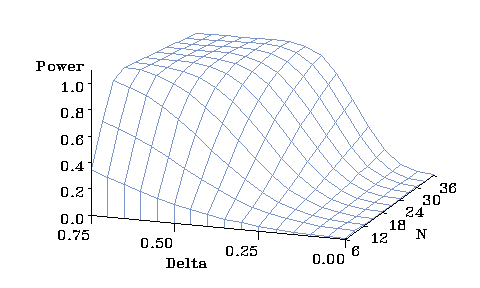
\includegraphics[width=4in]{TestConditionalTwoSampleTTest3DPlot.png}

\section*{References}

\hangindent2em
\hangafter=1
 Glueck, D. H., \& Muller, K. E. (2003). Adjusting power for a baseline covariate in linear models. \emph{Statistics in Medicine}, \emph{22}(16), 2535-2551.

\hangindent2em
\hangafter=1
 Johnson, J. L., Muller, K. E., Slaughter, J. C., Gurka, M. J., \& Gribbin, M. J. (2009). POWERLIB: SAS/IML Software for Computing Power in Multivariate Linear Models. \emph{Journal of Statistical Software}, \emph{30}(5), 1-27.

\hangindent2em
\hangafter=1
 Muller, K. E., \& Stewart, P. W. (2006). Linear model theory: univariate, multivariate, and mixed models. Hoboken, New Jersey: John Wiley and Sons.
\end{document}
